\documentclass[conference]{IEEEtran}
\IEEEoverridecommandlockouts
\pagestyle{plain}
\usepackage{amsmath,amssymb,amsfonts, mathtools}
\usepackage{algorithmic}
\usepackage{graphicx}
\usepackage{subcaption}
\usepackage[hidelinks]{hyperref}
\usepackage{textcomp}
\usepackage{xcolor}
\usepackage[inline]{enumitem}
\usepackage{minted}
\usepackage{tikz}
\usepackage{multicol}
\usetikzlibrary{calc,arrows.meta,positioning,arrows, automata, shapes}
\usepackage[
    backend=biber,
    style=alphabetic,
    citestyle=authoryear
]{biblatex}
\usepackage{csquotes}
\addbibresource{ref.bib}

\def\BibTeX{{\rm B\kern-.05em{\sc i\kern-.025em b}\kern-.08em
    T\kern-.1667em\lower.7ex\hbox{E}\kern-.125emX}}
    

\begin{document}
\title{
    Intrinsic Motivation Research in Reinforcement Learning
}

\author{\IEEEauthorblockN{
    Geert Goemaere
}
\IEEEauthorblockA{
    University of Antwerp \\
    geert.goemaere@student.uantwerpen.be}
}
\maketitle

\begin{abstract}
The field of Reinforcement Learning (RL) has managed to solve very complex tasks like video games or robotic tasks without human help. However, a huge weakness of RL remains when rewards are sparse or hard to get: an agent can only act randomly in hopes of discovering something rewarding. Researchers strive to generate interesting agents without rewards at all, a field sometimes called \textit{unsupervised RL}. These \textit{curious} agents often use intrinsic rewards to motivate exploration. I studied the theory behind the existing sub-fields and methods of Intrinsic Motivation, identified hindsight experience replay as branch of further research and explored ideas to improve learning with hindsight experience. I provided experiments in a gridworld setting and a robotic control setting to support my ideas. Based on those results, I propose possible areas of scientific research.
\end{abstract}

\section{Introduction}

In Reinforcement Learning (RL), an \textit{agent} gathers \textit{rewards} from an \textit{environment} while performing a task in that environment. The agent maximizes rewards by learning the optimal sequence of \textit{actions} while performing the task.

The reward may be a score when the agent learns to solve a game, or a distance function when the agent learns to reach a goal. In that case, the reward function is considered \textit{extrinsic}, i.e. provided by the environment specifically for the task. The agent learns by getting extrinsic rewards from the environment. Spectacular results have been obtained using extrinsic rewards on Atari game [\cite{bellemare2013arcade}] with Deep Q-network (DQN) [\cite{mnih2015human}] using deep reinforcement learning (DRL). 

When rewards are scattered or sparse in the environment, approaches relying on obtaining rewards from the environment are most of the time unsuccessful, as agent is not able to learn optimal actions for the targeted task. In addition, behaviour learned by an agent in one environment is hardly reusable in other environments whether it be for the same task or for other tasks. It is difficult for an agent to abstract or generalize decisions in an environment. Such abstract decisions could be: Take the key and go to the door. Those abstract decisions are performed by low-level actions moving in a certain direction, or picking-up an object by a robot controlling different joints. Those abstract decisions are often called \textit{options} [\cite{sutton1999between}]. To perform a certain task, agents often have to learn a set of tasks in a specific order. E.g. a robot grasping and object and putting it into a box should first learn how to grasp an object before it can learn how to put it into a box. There are potentially infinite number of those options in the real-world or a simulator (e.g. robotic tasks). This is an exploration problem in the option space rather than in the state space.

A limitation of deep reinforcement learning algorithms is their inability to learn a shared state representation independently from extrinsic rewards. Nevertheless, an agent could learn on other interesting features than the ground state space alone, allowing DRL algorithms to considerably speed up the learning process [\cite{raffin2019decoupling}].

Alternatively, unlike RL based on extrinsic rewards, developmental learning is based on the trend that babies, and in extension organisms, spontaneously explore the environment and acquire new skills. This is commonly called \textit{intrinsic motivation} (IM), which can be derived from an intrinsic reward. Intrinsic motivation allows learning new skills making the learning process of new tasks easier.

In this research project, I studied the theory behind intrinsic motivation in reinforcement learning by first understanding the lay of the land as provided by a survey on the role of intrinsic motivation in DRL. [\cite{aubret2019survey}]. As the research area is vast, I focus specifically on the skill learning branch, where \textit{hindsight experience replay} (HER) [\cite{andrychowicz2017hindsight}] as intrinsic motivation method will get most focus.

I believe the contribution of my work to to be
\begin{itemize}
    \item providing an overview on the landscape of intrinsic motivation in DRL
    \item charting the benefits of hindsight experience replay (HER) in DRL
    \item studying possible improvements on HER in tabular and deep settings
    \item proposing potential research areas to improve HER + DRL
\end{itemize}{}

In Section \ref{sec:literature_study}, I present related work, along with intrinsic motivation techniques and other approaches to learn from multiple signals. In Section \ref{sec:experiments}, I provide experiments in a tabular setting and deep setting to validate existing and proposed techniques. In Section \ref{sec:conclusion}, I discuss conclusions drawn from experiments. Finally, in Section \ref{sec:future_work}, I propose potential future work to explore and improve Intrinsic Motivation in Reinforcement Learning.

\section{Literature study} \label{sec:literature_study}

\subsection{A survey on intrinsic motivation in reinforcement learning}

This paper [\cite{aubret2019survey}] is a non-exhaustive review of current ongoing research directions, their limitations and their potential perspectives. The overall literature on IM is huge [\cite{barto2013intrinsic}] and the review only considers its application to DRL. It highlights how IM can improve over state-of-the-art DRL algorithms, scaling to large state and action dimension spaces.

Intrinsic Motivation addresses a number of challenges of standard RL:
\begin{itemize}
    \item Sparse rewards; The agent never receives rewards from the environment.
    \item State representation: The agent cannot learn a representation of its observations with independent features.
    \item Building option: The agent is unable to learn high-level decisions independent of the task.
    \item Learning curriculum: The agent can hardly learn a curriculum of subsequent tasks without expert knowledge.
\end{itemize}

IM offers a greater learning flexibility, through the use of a more general reward function, allowing to tackle the challenges raised above when only an extrinsic reward is used.

The RL framework can be reformulated, as done by [\cite{singh2010intrinsically}] and [\cite{barto2004intrinsically}], to incorporate IM. A distinction is made between a primary reward and a secondary reward signals. The primary reward signal is the standard extrinsic reward returned by the environment. The secondary signal is a local reward computed by the agent and thus internal or intrinsic to that agent. This new RL model can be seen in  Fig. \ref{fig:new_rl_model}.
\begin{figure}[h]
\centering
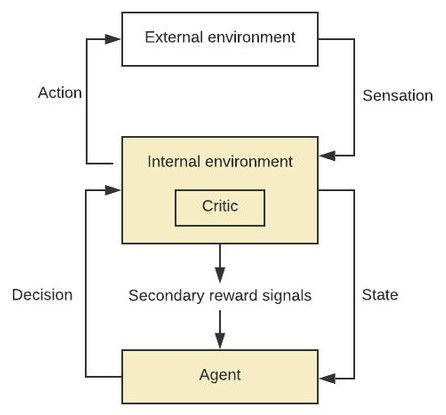
\includegraphics[width=0.9\columnwidth]{img/New-model-of-RL-integrating-IM-adapted-from-Singh-et-al-2010_W640.jpg}
\caption{New model of RL integrating IM, adapted from \cite{singh2010intrinsically}.}
\label{fig:new_rl_model}
\end{figure}

There are multiple ways to integrate an intrinsic reward into a RL framework. The main approach is to compute the agent’s reward r as a weighted sum
of an intrinsic reward $r_{int}$ and the extrinsic reward $r_{ext}$ [\cite{burda2018exploration}; \cite{gregor2016variational};\cite{vezhnevets2017feudal};\cite{huang2019learning}]:
\begin{equation*}
r = \alpha \cdot r_{int} + \beta \cdot r_{ext}
\end{equation*}

This paper [\cite{aubret2019survey} proposes a classification that emphasizes on two major kinds of intrinsic motivation in reinforcement learning: \textit{knowledge acquisition} explained in \ref{subsubsec:knowledge_acquisition}, and \textit{skill learning} detailed in \ref{subsubsec:skill_learning}. The classification is summarized in Table \ref{tab:classification}.

The large majority of research in the field is focused on knowledge acquisition. However, my interest is focused on skill learning and this was also the focus of my research project, both in subsequent literature study, experiments and ideas on future research work.

\begin{table}[h]
  \centering
  \begin{subtable}[t]{0.45\columnwidth}
    \centering
    \begin{tabular}{|p{0.90\textwidth}|}
      \hline
      \multicolumn{1}{|c|}{\textbf{Knowledge acquisition}} \\
      \hline
      \hline
      \textbf{Exploration} \\
      \hline
      Prediction error \\
      State novelty \\
      Novelty as discrepancy towards other states \\
      Information gain \\
      \hline
      \hline
      \textbf{Empowerment} \\
      \hline
      \hline
      \textbf{Learning a relevant state representation} \\
      \hline
      State space as a measure of distance \\
      One feature for one object of interaction \\
      \hline
    \end{tabular}
  \end{subtable}
  \hspace{0em}
  \begin{subtable}[t]{0.45\columnwidth}
    \centering
    \begin{tabular}{|p{0.90\textwidth}|}
      \hline
      \multicolumn{1}{|c|}{\textbf{Skill learning}} \\
      \hline
      \hline
      \textbf{Skill abstraction} \\
      \hline
      Building the goal space from the state space \\
      Mutual information between goals and trajectories \\
      \hline
      \hline
      \textbf{Curriculum learning} \\
      \hline
      Goal sampling \\
      Multi-armed bandit \\
      Adversarial training \\
      \hline
    \end{tabular}
  \end{subtable}
  \caption{Classification of the use of IM in DRL.}
  \label{tab:classification}
\end{table}

\subsubsection{Knowledge acquisition} \label{subsubsec:knowledge_acquisition}
The agent strives to find new knowledge about its environment. Knowledge acquisition can improve \textbf{exploration} in sparse reward environments by computing intrinsic reward e.g. based on novelty of states or information gain. There are three main methods tackling exploration. The first is \textit{prediction error}. The agent is steered to areas where prediction of a state following a state-action tuple is difficult. The second method is \textit{state novelty} where the agent goes into states in which it usually never goes. This method is count-based, i.e. as an agent visits  a state, the intrinsic reward associated with that state decreases. A third method is \textit{information gain}, which is a reward based on reduction of uncertainty on the environment dynamics. This pushes the agent towards areas it does not know, but also prevents attraction to stochastic areas. The exploration problem is probably the largest use case for IM. An agent maximizing \textbf{empowerment} tries to have most control on its environment. This method can be used to avoid an extrinsic award but the main difficulty is its complexity. Several approaches use an environment model to compute rewards based in empowerment, but the essence of RL is that the agent does not know the environment dynamics or reward function a priori. Existing work in this area remains limited. \textbf{Learning a relevant state representation} is the ability of an agent to project its raw state  onto a feature space with meaningful properties. Two different sets of work can be identified. The first, \textit{state space as a measure of distance}, tries to fit distance in the representation space where distance is expressed in terms of actions in the state space. The seconds set, \textit{one feature for one object of interaction}, tries to learn independent factors of variation in the embedding space. A goal is presented as a variation of a one feature in the embedding space, which is learnt simultaneously with the policy controlling the feature [\cite{thomas2017independently}]. E.g., a feature can be a light in a room where a policy relative to a factor of variation can be switching the lamp on or off. The reward is maximized by finding the optimal set of policies.

\subsubsection{Skill learning} \label{subsubsec:skill_learning}
The agent's ability to construct task-independent and reusable skills in an efficient way. \textbf{Skill abstraction} is the ability of an agent to learn a representation of diverse skills. Skills or goals generated by an agent are also called \textit{options}. Skills are learned in an unsupervised way. The agent generates options and learns associated intra-options policies using intrinsic rewards. If a global task exists, the agent will learn to use its skills to realize a global objective using extrinsic rewards associated with that task. To learn intra-options policies it is possible to use hindsight experience replay [\cite{andrychowicz2017hindsight}] because a reward function can be computed without additional interactions if only an intrinsic reward is used. It is key to learn interesting skills that can be transferred between different tasks. there are two main research directions on self-generation of goals. The first one is about \textit{building the goal space from the state space}. It considers its objectives as states in which the agent is required to find the right distance measure and right way to compress the state space to let an inter-option policy generate high-dimensional actions and discern similar states from different states. The second area is about using \textit{mutual information between goals and trajectories} to generate skills based on a diversity heuristic. It is about learning skills according to the ability of the agent to discern skills from the trajectory of the intra-options policy. The agent goes into areas for which it can guess the option it has chosen. The aim of \text{curriculum learning} is to learn to choose an objective which speeds up learning of several goals of an agent. To be efficient, the curriculum must avoid forgetting what has already been learned and avoid trying to learn unlearnable tasks. Several techniques exist to select goals to learn learned and act upon. \textit{Simple goal sampling} is a simple way to select goals based on some strategy. For example, HER [\cite{andrychowicz2017hindsight}] proposes four different strategies to choose the goal to replace in transition experience. These are explained in \ref{subsec:her}. Another common way to choose a task is \textit{task selection as a multi-armed bandit}, which associates a learning progress value to each task. The agent will choose the task using its estimated learning progress and tries to solve the task with the task-specific reward. This is harder when the task is continuously parameterized. \textit{Task selection with adversarial training} can overcome the need for a discrete goal space. In the paradigm of adversarial training, a generator learns to generate goals and a discriminator learns to distinguish these goals from others. Adversarial methods can learn with a continuous goal space but need a good goal representation.

\subsection{Hindsight Experience Replay} \label{subsec:her}
This paper [\cite{andrychowicz2017hindsight}] proposes a novel technique called Hindsight Experience Replay (HER) which allows sample-efficient learning from rewards which are sparse and binary and avoids the need for complicated reward engineering. The idea is that an agent can also learn from episodes where the goal has not been reached. The algorithm is as follows:
\begin{itemize}
\item During training, after experiencing some episode while acting in the environment:
\item For each transition in such an episode
\begin{itemize}
    \item store the transition in a replay buffer
    \item sample a goal from the episode according to some strategy
    \item duplicate the transition, replace the goal with the sampled goal and store the duplicate transition in the replay buffer
\end{itemize}
\item Train policies and value functions with transitions sampled from the replay buffer 
\end{itemize}
[\cite{andrychowicz2017hindsight}] proposes four different strategies to choose a goal from the current episode to replace the goal in the transitions of an episode;
\begin{itemize}
 \item \texttt{Final} - choose final state of same episode as transition being replayed
 \item \texttt{Future} - choose set of random states from same episode as transition being replayed and observed after replayed transition
 \item \texttt{Episode} - choose set of random states from same episode as transition being replayed 
 \item \texttt{Random} - choose set of random states encountered so far during training
\end{itemize}

\begin{figure}[ht]
\centering
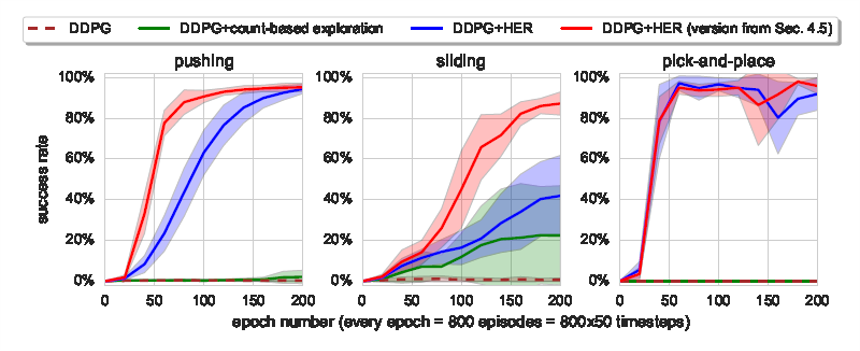
\includegraphics[width=0.9\columnwidth]{img/HER_robotic_experiments.png}
\caption{Learning curves for multi-goal setup in case of DDPG with and without HER. DDPG with HER solves the task confirming that HER is crucial for learning from sparse, binary rewards.}
\label{fig:her_robot_experiment}
\end{figure}
Experiments reported in [\cite{andrychowicz2017hindsight}] and shown in Fig. \ref{fig:her_robot_experiment} indicate that HER enables RL to use spare rewards combined with off-policy algorithms. Robotic arm experiments show that trained policies in simulation perform well in real-life without fine-tuning (trained with off-policy RL algorithm).
HER enables RL algorithms to use sparse rewards. A limitation of HER is that it can be applied as long as a goal space can be defined from a state space. HER may be seen as a form of implicit curriculum as the goals used for replay naturally shift from ones which are simple to achieve even by a random agent to more difficult ones.

\subsection{The Option-Critic Architecture}
Temporal abstraction allows representing knowledge about courses of action that take place at different time scales. In reinforcement learning, options [\cite{sutton1999between}]] provide a framework for defining such courses of action and for seamlessly learning and planning with them. Based on the policy gradient theorem [\cite{sutton2000policy}], the proposal in [\cite{bacon2017option}] derives new results which enable a gradual learning process of intra-option policies and termination functions, simultaneously with the policy over them. This approach works naturally with both linear and non-linear function approximators, under discrete or continuous state and action spaces. The option critic architecture as proposed by [\cite{bacon2017option}] is shown in Fig. \ref{fig:option_critic_arch}. 
\begin{figure}[ht]
\centering
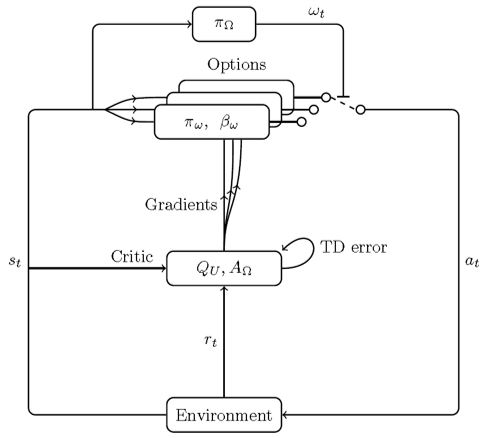
\includegraphics[width=0.9\columnwidth]{img/OptionCriticArch.png}
\caption{Diagram of the option-critic architecture. The option execution model is depicted by a \textit{switch} $\perp$ over the \textit{contacts} $\multimap$. A new option is selected according to $\pi_{\Omega}$ only when the current option terminates.}
\label{fig:option_critic_arch}
\end{figure}

The option-critic architecture works according to a \textit{call-and-return option execution model}:
\begin{enumerate}
    \item Agent picks option $\omega$ according to an inter-option policy $\pi_{\Omega}$
    \item Agent then follows an intra-option policy $\pi_{\omega}$ until termination ($\beta_{\omega}$)
    \item Repeat procedure
\end{enumerate}
The proposal in [\cite{bacon2017option}] developed a general gradient-based approach for learning simultaneously the intra-option policies and termination functions, as well as the policy over options, in order to optimize a performance objective for the task at hand.

\subsection{Learning Multi-Level Hierarchies with Hindsight}
Multi-level hierarchies have the potential to accelerate learning in sparse reward tasks because they can divide a problem into a set of short horizon sub-problems. The proposal in [\cite{levy2019learning}] introduces a framework that can learn multiple levels of policies in parallel, so the simpler sub-problems can be solved simultaneously. The framework, called \textit{hierarchical actor-critic} (HAC), has a hierarchical architecture and a method for learning multiple levels of goal-conditioned policies in parallel given sparse rewards. The number of levels in the hierarchy is a hyperparameter chosen by the user.
-
The highest level policy takes as input the current state and goal state provided by the task and outputs a sub-goal state. This state is used as the goal state for the policy at the next level down. The policy at that level takes as input the current state and the goal state provided by the level above and outputs its own sub-goal state for the next level below to achieve. This process continues until the lowest level is reached. The lowest level then takes as input the current state and the goal state provided by the level above and outputs a primitive action. Further, each level has a certain number of attempts to achieve its goal state. When the level either runs out of attempts or achieves its goal state, execution at that level ceases and the level above outputs another sub-goal. Fig. \ref{fig:mutilevel_her_example} shows an example of an agent using a 3-level policy hierarchy to move through rooms to reach its target.
\begin{figure}[ht]
\centering
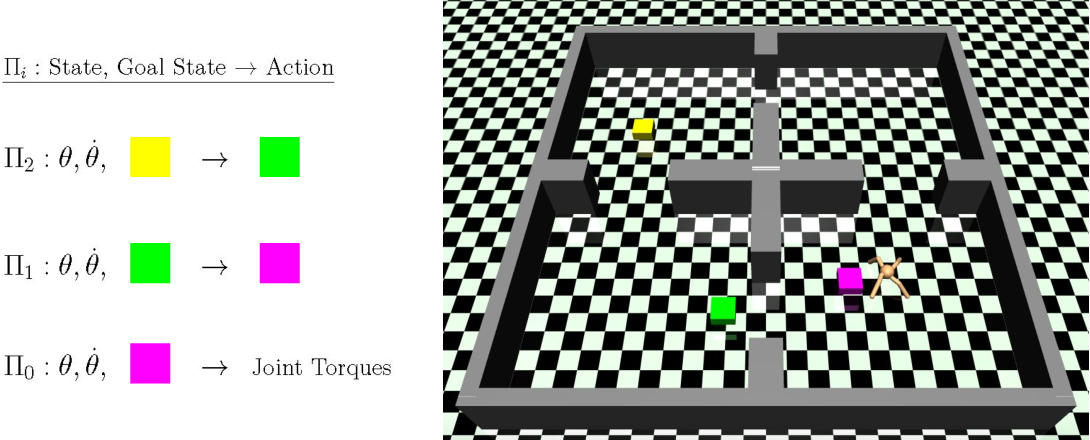
\includegraphics[width=0.9\columnwidth]{img/MultiLevelHER_example.png}
\caption{An ant agent uses a 3-level hierarchy to traverse though rooms to reach its goal, represented by the yellow cube. $\Pi_2$ uses as input the current state (joint positions $\theta$ and velocities $\dot{\theta}$) and goal state (yellow box) and outputs a sub-goal state (green box) for $\Pi_1$ to achieve. $\Pi_1$ takes in the current state and its goal state (green box) and outputs a sub-goal state (purple box) for $\Pi_0$ to achieve. $\Pi_0$ takes in the current state and goal state (purple box) and outputs a vector of joint torques}
\label{fig:mutilevel_her_example}
\end{figure}

Experiments in [\cite{levy2019learning}] compare performance of agents using policy hierarchies with 1 (i.e., flat) and more levels with agents using Q-learning [\cite{watkins1992q}] with HER in discrete tasks and DDPG [\cite{lillicrap2015continuous}] with HER in the continuous tasks. The empirical results show that the HAC framework can benefit from additional levels of hierarchy and that multi-level agents outperform flat agents.

\section{Experiments} \label{sec:experiments}
Literature study made it clear to me that hindsight experience replay is a key method to improve training of agents in sparse reward settings. In my experiments, I implemented HER in a Q-learning agent and measured training performance in a tabular gridworld setting. I compared the results of tabular Q-learning with HER to a baseline of tabular Q-learning without HER. From there, I tried to improve performance using new ideas. I also did experiments with HER for a robotic control task to verify whether performance of hindsight experience replay would translate to a deep learning setting.

\subsection{Tabular Q-Learning with hindsight} \label{subsec:exp_tab_her}
For this experiment, the task for the agent is to reach a position in a four-room environment in as few steps as possible. I used a small 3x3 \texttt{FourRoomsGoal-v0} environment and a larger 10x10 \texttt{FourRoomsGoalBig-v0} environment are used to compare how scaling up influences training efficiency. Both rooms are goal-oriented variations on the Minimalistic Gridworld Environment in [\cite{gym_minigrid}]. Fig. \ref{fig:tabular_fourroomsgoal_env} shows the \texttt{FourRoomsGoal-v0} environment.
\begin{figure}[ht]
\centering
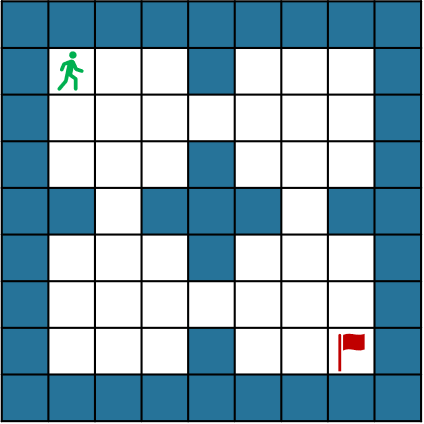
\includegraphics[width=0.5\columnwidth]{img/FourRoomsGoal-v0.png}
\caption{Goal-oriented 3x3 FourRoomsGoal-v0 environment.}
\label{fig:tabular_fourroomsgoal_env}
\end{figure}
The setting of the experiment is:
\begin{itemize}
    \item Each training episode has random start and goal position.
    \item A sparse reward $r = 1$ is returned if goal (red flag) is reached or $r = 0$ otherwise.
\end{itemize}
In Q-learning an agent learns from every transition. During this experiment, an agent continues an episode and only stops when the goal has been reached.
In the hindsight experience replay experiments as defined in [\cite{andrychowicz2017hindsight}], good results were obtained using a \texttt{final} goal-sampling strategy where the final state in an episode is used for goal replacement in all experienced transitions of that episode. I use a slight variation on this algorithm in that I device an episode into \textbf{subtraject} where for all transitions in that subtraject the \texttt{final} state of that subtraject is selected for goal replacement. The subtraject length is an hyperparameter then and using a grid search I tried to find the length which results in the optimal performance, i.e. the least number of steps to reach the goal state. The resulting algorithm for tabular Q-Learning with hindsight is then:
\begin{itemize}
\item Episodes are divided in sub-trajects
\item For each transition in sub-traject
    \begin{itemize}
    \item Store the transition in a replay buffer
    \item Sample the final goal from sub-traject and replace each goal in a duplicate of the transition
    \item Store the modified duplicate in the replay buffer
    \end{itemize}
\item For each episode, sample a mini-batch of transitions from the replay buffer
\item Update the agent's QA-table with the sampled transitions
\end{itemize}
The results of tabular Q-Learning with and without hindsight experience in the \textit{3x3 FourRoomsGoal-v0} environment are shown in Fig. \ref{fig:experiment_fourroomsgoal_learning_performance}.

\begin{figure}[ht]
\centering
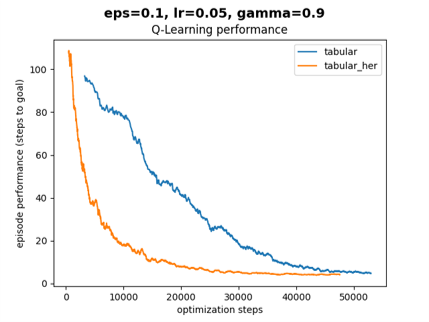
\includegraphics[width=0.9\columnwidth]{img/exp_tabular_her_fourroom_small.png}
\caption{Learning curve of tabular Q-learning with and without HER for the 3x3 FourRoomsGoal-v0 environment. The performance is measured in number of episode steps required to reach target in function of optimization steps of the Q-learning agent. The results show the average performance over 10 runs of 3000 episodes each. The sub-trajectory length for Q-learning with HER equals 28 steps.}
\label{fig:experiment_fourroomsgoal_learning_performance}
\end{figure}

It's clear that Q-learning with HER outperforms Q-learning without HER. HER has faster learning and converges faster using less optimization steps. The reason for measuring performance in function of optimization steps and not in function of the number of episodes is to have a more honest comparison between HER and non-HER experiments. HER can do more optimizations per episode because it samples mini-batches of transitions from the experience replay buffer. In Fig. \ref{fig:experiment_fourroomsgoal_learning_performance} a clear \textit{shift} to the right of both curves can be noticed. This artifact is due to a smoothing algorithm which smooths results over 30 periods. This shift is less pronounced for HER because it learns faster and quickly requires less optimization steps per episode. The learning curve converges to a value of about 6 steps. This is on average the distance between the randomly assigned start and goal positions. Best case this distance is 1 step and worst case it is 12 steps.

The results of tabular Q-Learning with and without hindsight experience in the \textit{10x10 FourRoomsGoalBig-v0} environment are shown in Fig. \ref{fig:experiment_fourroomsgoalbig_learning_performance}. It's clear that Q-learning with HER clearly outperforms Q-learning without HER. The difference is even more pronounced that in the smaller environment. Again HER converges faster than non-HER as HER does more optimizations per episode. The HER learning curve seems to converge to a value towards 200 although the curve is not yet flat after 3 million optimization steps. In the bigger fourrooms environment, best case distance is 1 step and worst case distance is 40 steps. On average this would lead to an optimal value of 20 steps. An explanation to the difference between the actual curve and optimal value could be that the agent's '$\epsilon$-greedy algorithm part of the time still explores and doesn't always choose the best action. 
\begin{figure}[ht]
\centering
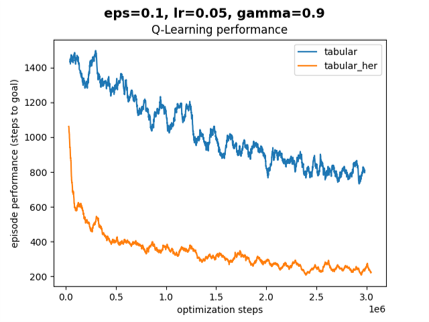
\includegraphics[width=0.9\columnwidth]{img/exp_tabular_her_fourroom_big.png}
\caption{Learning curve of tabular Q-learning with and without HER for the 10x10 FourRoomsGoalBig-v0 environment. The performance is measured in number of episode steps required to reach target in function of optimization steps of the Q-learning agent. The results show the average performance over 10 runs of 20000 episodes each. The sub-trajectory length for Q-learning with HER equals 44 steps.}
\label{fig:experiment_fourroomsgoalbig_learning_performance}
\end{figure}

As mentioned before, I use a variation of the HER algorithm in which episodes are divided into subtrajects with the subtraject length used as a hyperparameter. I performed a grid search for both environments used in the experiments to find the optimal value, i.e. a subtraject length that minimizes the number of steps needed to reach the goal position in the fourroom environments. The results of this grid search are shown in Fig. \ref{fig:experiment_subtraject_gridsearch}. 

\begin{figure}[ht]
\centering
\begin{subfigure}[t]{0.45\columnwidth}
\centering
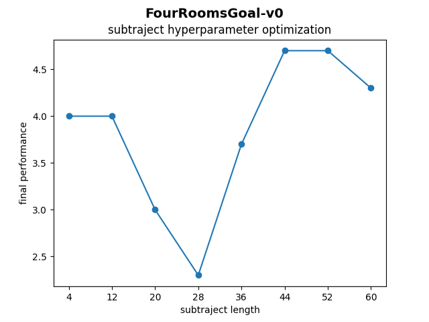
\includegraphics[width=1.0\textwidth]{img/exp_tabular_her_gridsearch_small.png}
\caption{FourRoomsGoal-v0 performance in function of subtraject length.}
\label{fig:experiment_subtraject_gridsearch_small}
\end{subfigure}
\hspace{0em}
\begin{subfigure}[t]{0.45\columnwidth}
\centering
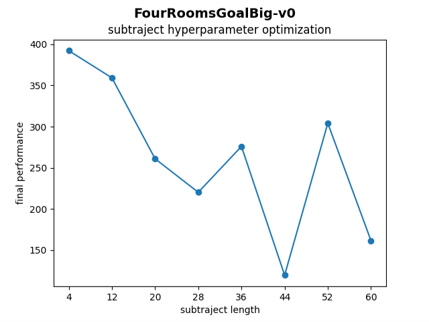
\includegraphics[width=1.0\textwidth]{img/exp_tabular_her_gridsearch_big.png}
\caption{FourRoomsGoalBig-v0 performance in function of subtraject length.}
\label{fig:experiment_subtraject_gridsearch_big}
\end{subfigure}
\caption{Grid search results on the optimal hyperparameter subtraject length parameter.}
\label{fig:experiment_subtraject_gridsearch}
\end{figure}

Although the plots are somewhat noisy due to the coarse granularity of subtraject values in the grid search, a clear trend can be noticed. For the \textit{FourRoomsGoal-v0} environment (Fig. \ref{fig:experiment_subtraject_gridsearch_small}) an optimal value of 28 was found and for the \textit{FourRoomsGoalBig-v0} environment (Fig. \ref{fig:experiment_subtraject_gridsearch_big}) this value was 44. To be sure that the values are not local minima, a more extensive grid search would be required.

\subsection{Option Learning with Hindsight}
Knowing that we can train a Q-learning agent with HER and that it greatly improves learning over non-HER Q-learning, can we also use that agent for more complex tasks than just reaching a goal? Suppose we have an environment where we can only reach a goal if certain sub-goals are reached first. Suppose further that a meta-agent exists that can learn high-level goals (options) and a controller agent that knows how to perform low-level actions to actually reach goals. The meta-agent only knows when a final goal has been reached when it receives a sparse reward. Fig. \ref{fig:experiment_option_her_concept} shows the concept.

\begin{figure}[ht]
\centering
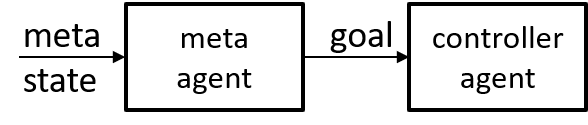
\includegraphics[width=0.9\columnwidth]{img/option_her_concept.png}
\caption{Option learning meta-agent using a controller agent to reach goals.}
\label{fig:experiment_option_her_concept}
\end{figure}

In this experiment, I created an \textit{FourRoomsKeyDoorEnv-v0} environment with a key and a door. The environment is very similar to the \textit{FoorRoomsGoalEnv-v0} used in \ref{subsec:exp_tab_her}, with the difference that the goal is to reach the door while having a key. The options to discover are the key and the door. I created two variants of this environment: \textit{FourRoomsKeyDoorEnv-v0} and \textit{FourRoomsBigKeyDoorEnv-v0} to assess training in small and big room environments. Fig. \ref{fig:experiment_option_her_keydoor_env} shows the \textit{FourRoomsKeyDoorEnv-v0} environment.

\begin{figure}[ht]
\centering
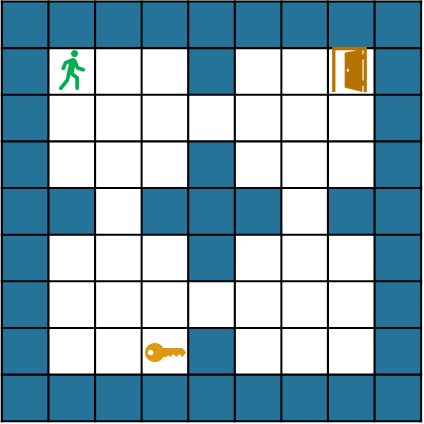
\includegraphics[width=0.5\columnwidth]{img/FourRoomsKeyDoorEnv-v0.png}
\caption{3x3 FourRoomsKeyDoorEnv-v0 environment.}
\label{fig:experiment_option_her_keydoor_env}
\end{figure}

The setting of the experiment is as follows:
\begin{description}
\item[Environment] Four rooms with key and door placed at fixed position. The observation space is described by (position, key) with key as picked-up flag. The reward function is $r = (key==1 \And position==door)$
\item[Meta-agent] Q-Learning agent. The meta-agent trains a policy to select the best goal, based on the state, i.e. key being picked up or not. The high-level goals learned are actually the options used as sub-goals for the controller agent. 
\item[Controller-agent] Q-Learning with HER agent. The controller agent is pretrained to reach goals. It's policy is trained on state described by (position, goal) and its low-level actions are basic movements \texttt{up, down, left, right}.
\end{description}

With the described setting it's straight forward to train the meta-agent as a Q-learning agent. Options are generated according to an $\epsilon$-greedy policy, while the controller agent is acting greedy according to its pretrained policy. The training performance of the meta-agent is shown in Fig. \ref{fig:exp_option_her_training_small} for the small environment.  The learning curve shows the number of options or high-level goals taken to reach the door with the key. It converges to slightly above 2 options (optimal is 2, i.e. the key and door option). The agent still explores explaining why on average the number is slightly above 2. Fig. shows the training performance \ref{fig:exp_option_her_training_big} for the big environment. Similar results are obtained.

\begin{figure}[ht]
\centering
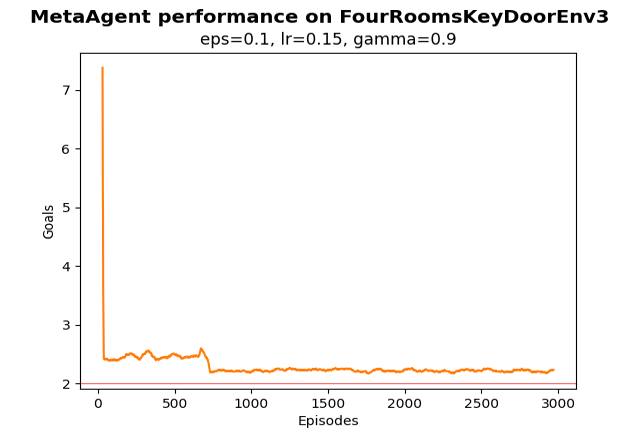
\includegraphics[width=0.9\columnwidth]{img/exp_option_her_keydoor_small.png}
\caption{Learning curve of meta-agent option learning for the FourRoomsKeyDoorEnv environment. The performance is measured in number of options needed to reach target in function of episode. Results are averaged over 10 training runs of 3000 episodes each.}
\label{fig:exp_option_her_training_small}
\end{figure}

\begin{figure}[ht]
\centering
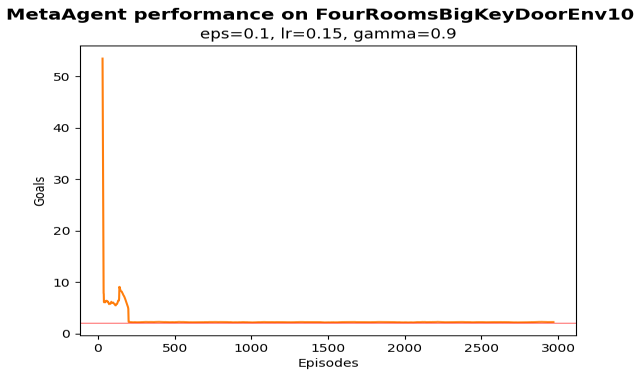
\includegraphics[width=0.9\columnwidth]{img/exp_option_her_keydoor_big.png}
\caption{Learning curve of meta-agent option learning for the FourRoomsBigKeyDoorEnv environment. The performance is measured in number of options needed to reach target in function of episode. Results are averaged over 10 training runs of 3000 episodes each.}
\label{fig:exp_option_her_training_big}
\end{figure}

As the meta-agent only has two states and as many actions as potential goals, equaling the state space, the agent conceptually learns in two different Qtable planes, one where the key hasn't been picked up yet, and one where the key has been picked up. These Qtable planes are shown for the \textit{FourRoomsKeyDoorEnv} environment in Fig. \ref{fig:exp_option_her_qtable_small_key0} (key not picked up) and in Fig. \ref{fig:exp_option_her_qtable_small_key1} where the key has been picked up. Looking at the state-action values in Fig. \ref{fig:exp_option_her_qtable_small_key0}, its clear that the best option to take is goal position where the key is located in case it hasn't been picked up yet. Looking at Fig. \ref{fig:exp_option_her_qtable_small_key1}, the best option to take is the door position in case the key has been picked up. We can conclude that the meta-agent has learned the best options to perform the task optimally. Results for the bigger \textit{FourRoomsBigKeyDoorEnv} environment are similar and the same two options are discovered.

\begin{figure}[ht]
\centering
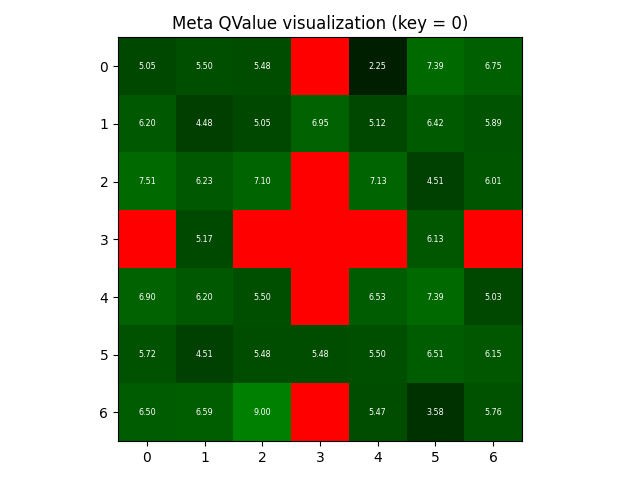
\includegraphics[width=0.9\columnwidth]{img/exp_option_her_qtable_small_key0.png}
\caption{Qtable of the option learning meta-agent for the FourRoomsKeyDoorEnv environment.}
\label{fig:exp_option_her_qtable_small_key0}
\end{figure}

\begin{figure}[ht]
\centering
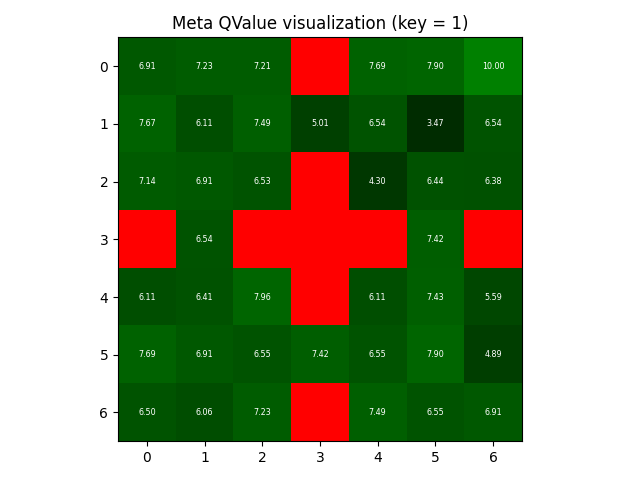
\includegraphics[width=0.9\columnwidth]{img/exp_option_her_qtable_small_key1.png}
\caption{Qtable of the option learning meta-agent for the FourRoomsKeyDoorEnv environment.}
\label{fig:exp_option_her_qtable_small_key1}
\end{figure}

After being trained, according to the meta-agent's Qtable values, it should perform optimal. The results of test runs with the trained meta-agent confirm this claim. Fig. \ref{fig:exp_option_her_test_perf_small} shows that the meta-agent only needs two high-level options to reach the door with the key for the small \textit{FourRoomsKeyDoorEnv}. Fig. \ref{fig:exp_option_her_test_pick_small} gives the chance that the key was picked up by accident, i.e. that a goal was chosen by the meta-agent which lead the controller agent over a path containing the key position but not landing on the key position. This would mean the key was picked up by chance, rather than following an optimal policy. As can be seen, this was not the case during test. Similar results where obtained for the bigger  \textit{FourRoomsBigKeyDoorEnv} environment.

\begin{figure}[ht]
\centering
\begin{subfigure}[t]{0.45\columnwidth}
\centering
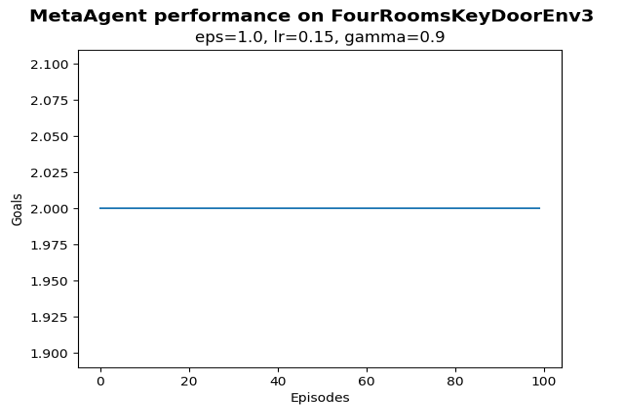
\includegraphics[width=1.0\textwidth]{img/exp_option_her_test_perf_small.png}
\caption{FourRoomsKeyDoorEnv-v0 meta-agent performance as number of options to target per test episode.}
\label{fig:exp_option_her_test_perf_small}
\end{subfigure}
\hspace{0em}
\begin{subfigure}[t]{0.45\columnwidth}
\centering
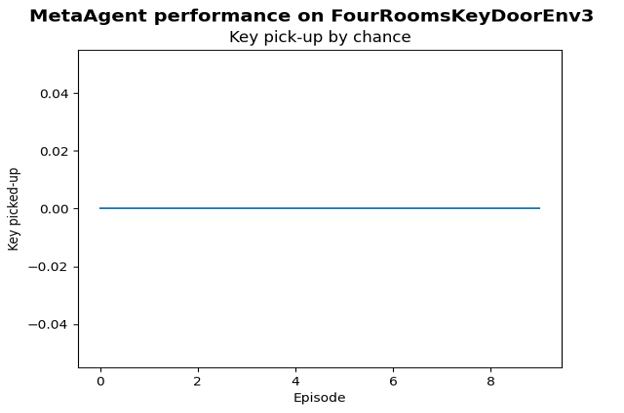
\includegraphics[width=1.0\textwidth]{img/exp_option_her_test_pick_small.png}
\caption{FourRoomsKeyDoorEnv-v0 meta-agent ‘key pick-up by chance’ incidence per test episode.}
\label{fig:exp_option_her_test_pick_small}
\end{subfigure}
\caption{FourRoomsKeyDoorEnv-v0 meta-agent test performance.}
\label{fig:exp_option_her_test_small}
\end{figure}

This experiment showed that we can train a Q-learning meta-agent to discover options to give to a pretrained controller agent performing the low-level actions to reach those options in order to perform more complex tasks than just reaching a single goal, and this in sparse reward setting using intrinsic motivation. 

\subsection{From tabular to deep learning for motor control task}


\section{Conclusion} \label{sec:conclusion}
\section{Future work} \label{sec:future_work}

\newpage
\printbibliography
\end{document}